\documentclass[a4paper]{article}
\usepackage[letterpaper, margin=1in]{geometry} % page format
\usepackage{listings} % this package is for including code
\usepackage{graphicx} % this package is for including figures
\usepackage{amsmath}  % this package is for math and matrices
\usepackage{amsfonts} % this package is for math fonts
\usepackage{tikz} % for drawings

\title{Homework 0}
\author{Colin May}
\date{}

\begin{document}
\lstset{language=Python}

\maketitle

\section{Python Requirements}

\includegraphics[scale=0.5]{PythonPackages}

\section{Github}
Github username: data440may 

Github link: https://github.com/colinomay/data440may


\includegraphics[scale=0.5]{collabinvite}

\section{Kaggle}
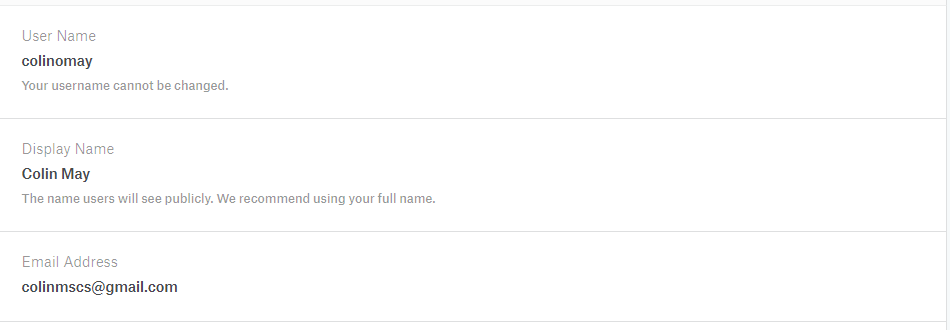
\includegraphics{kaggle}

\section{Problems}
\subsection{}
For the function $g(x) = −3x^2 + 24x - 30$, find the value for x that maximizes g(x): \\\\
\indent
$g(4) = 18$
\subsection{}
Consider the following function: $f(x) = 3x^3_0 - 2x_0x^2_1 + 4x_1 - 8$, what are the partial derivatives of $f(x)$ with respect to $x_0$ and $x_1$. \\\\
\indent
$9x^2-4x_0x$
\subsection{}
(a) can you multiply the two matrices? elaborate on your answer: \\
\indent
No, because A is a 2x3 and B is also a 2x3 matrix, multiplication isn't possible. \\
(b)  multiply $A^T$ and B and give its rank.
$$
\quad
\begin{bmatrix} 
-2 & -2 & 13 \\
8 & 1 & 16 \\
6 & -3 & -3
\end{bmatrix}
$$ 
\begin{center}
   Rank = 2 \\ 
\end{center}
(c)  what is the result of $AB^T + C^-1$?
$$
\quad
\begin{bmatrix} 
15 & 15 \\
-12 & -16
\end{bmatrix}
$$
\begin{lstlisting}[frame=single]
import numpy as np

A = np.array([[1,4,-3],[2,-1,3]])
B = np.array([[-2,0,5],[0,-1,4]])

# (a)
#np.dot(A,B) 

# (b)
np.dot(A.T,B)
np.linalg.matrix_rank(np.dot(A.T,B))

# (c)
C = np.array([[1,0],[0,2]])
np.dot(A,B.T)+C^-1
\end{lstlisting}
\subsection{}
Simple Gaussian: the normal distribution with a mean of zero and a variance of one (the green curves in the plots to the right). It is often called the bell curve because the graph of its probability density looks like a bell. \\

Multivariate Gaussian: a generalization of the one-dimensional normal distribution to higher dimensions. \\

Bernoulli: the discrete probability distribution of a random variable which takes the value 1 with probability p and the value 0 with probability q=1-p. \\

Binomial: the discrete probability distribution of the number of successes in a sequence of n independent experiments. \\

Exponential: the probability distribution of the time between events in a Poisson point process, i.e., a process in which events occur continuously and independently at a constant average rate.

\subsection{}
A Bernoulli random variable has two possible outcomes: 0 or 1. A binomial distribution is the sum of independent and identically distributed Bernoulli random variables.

\subsection{}
$X \sim N(2,3) = -7<X<11$

\subsection{}
\subsection{}

\end{document}
